\begin{figure*}[htbp]
    \centering
    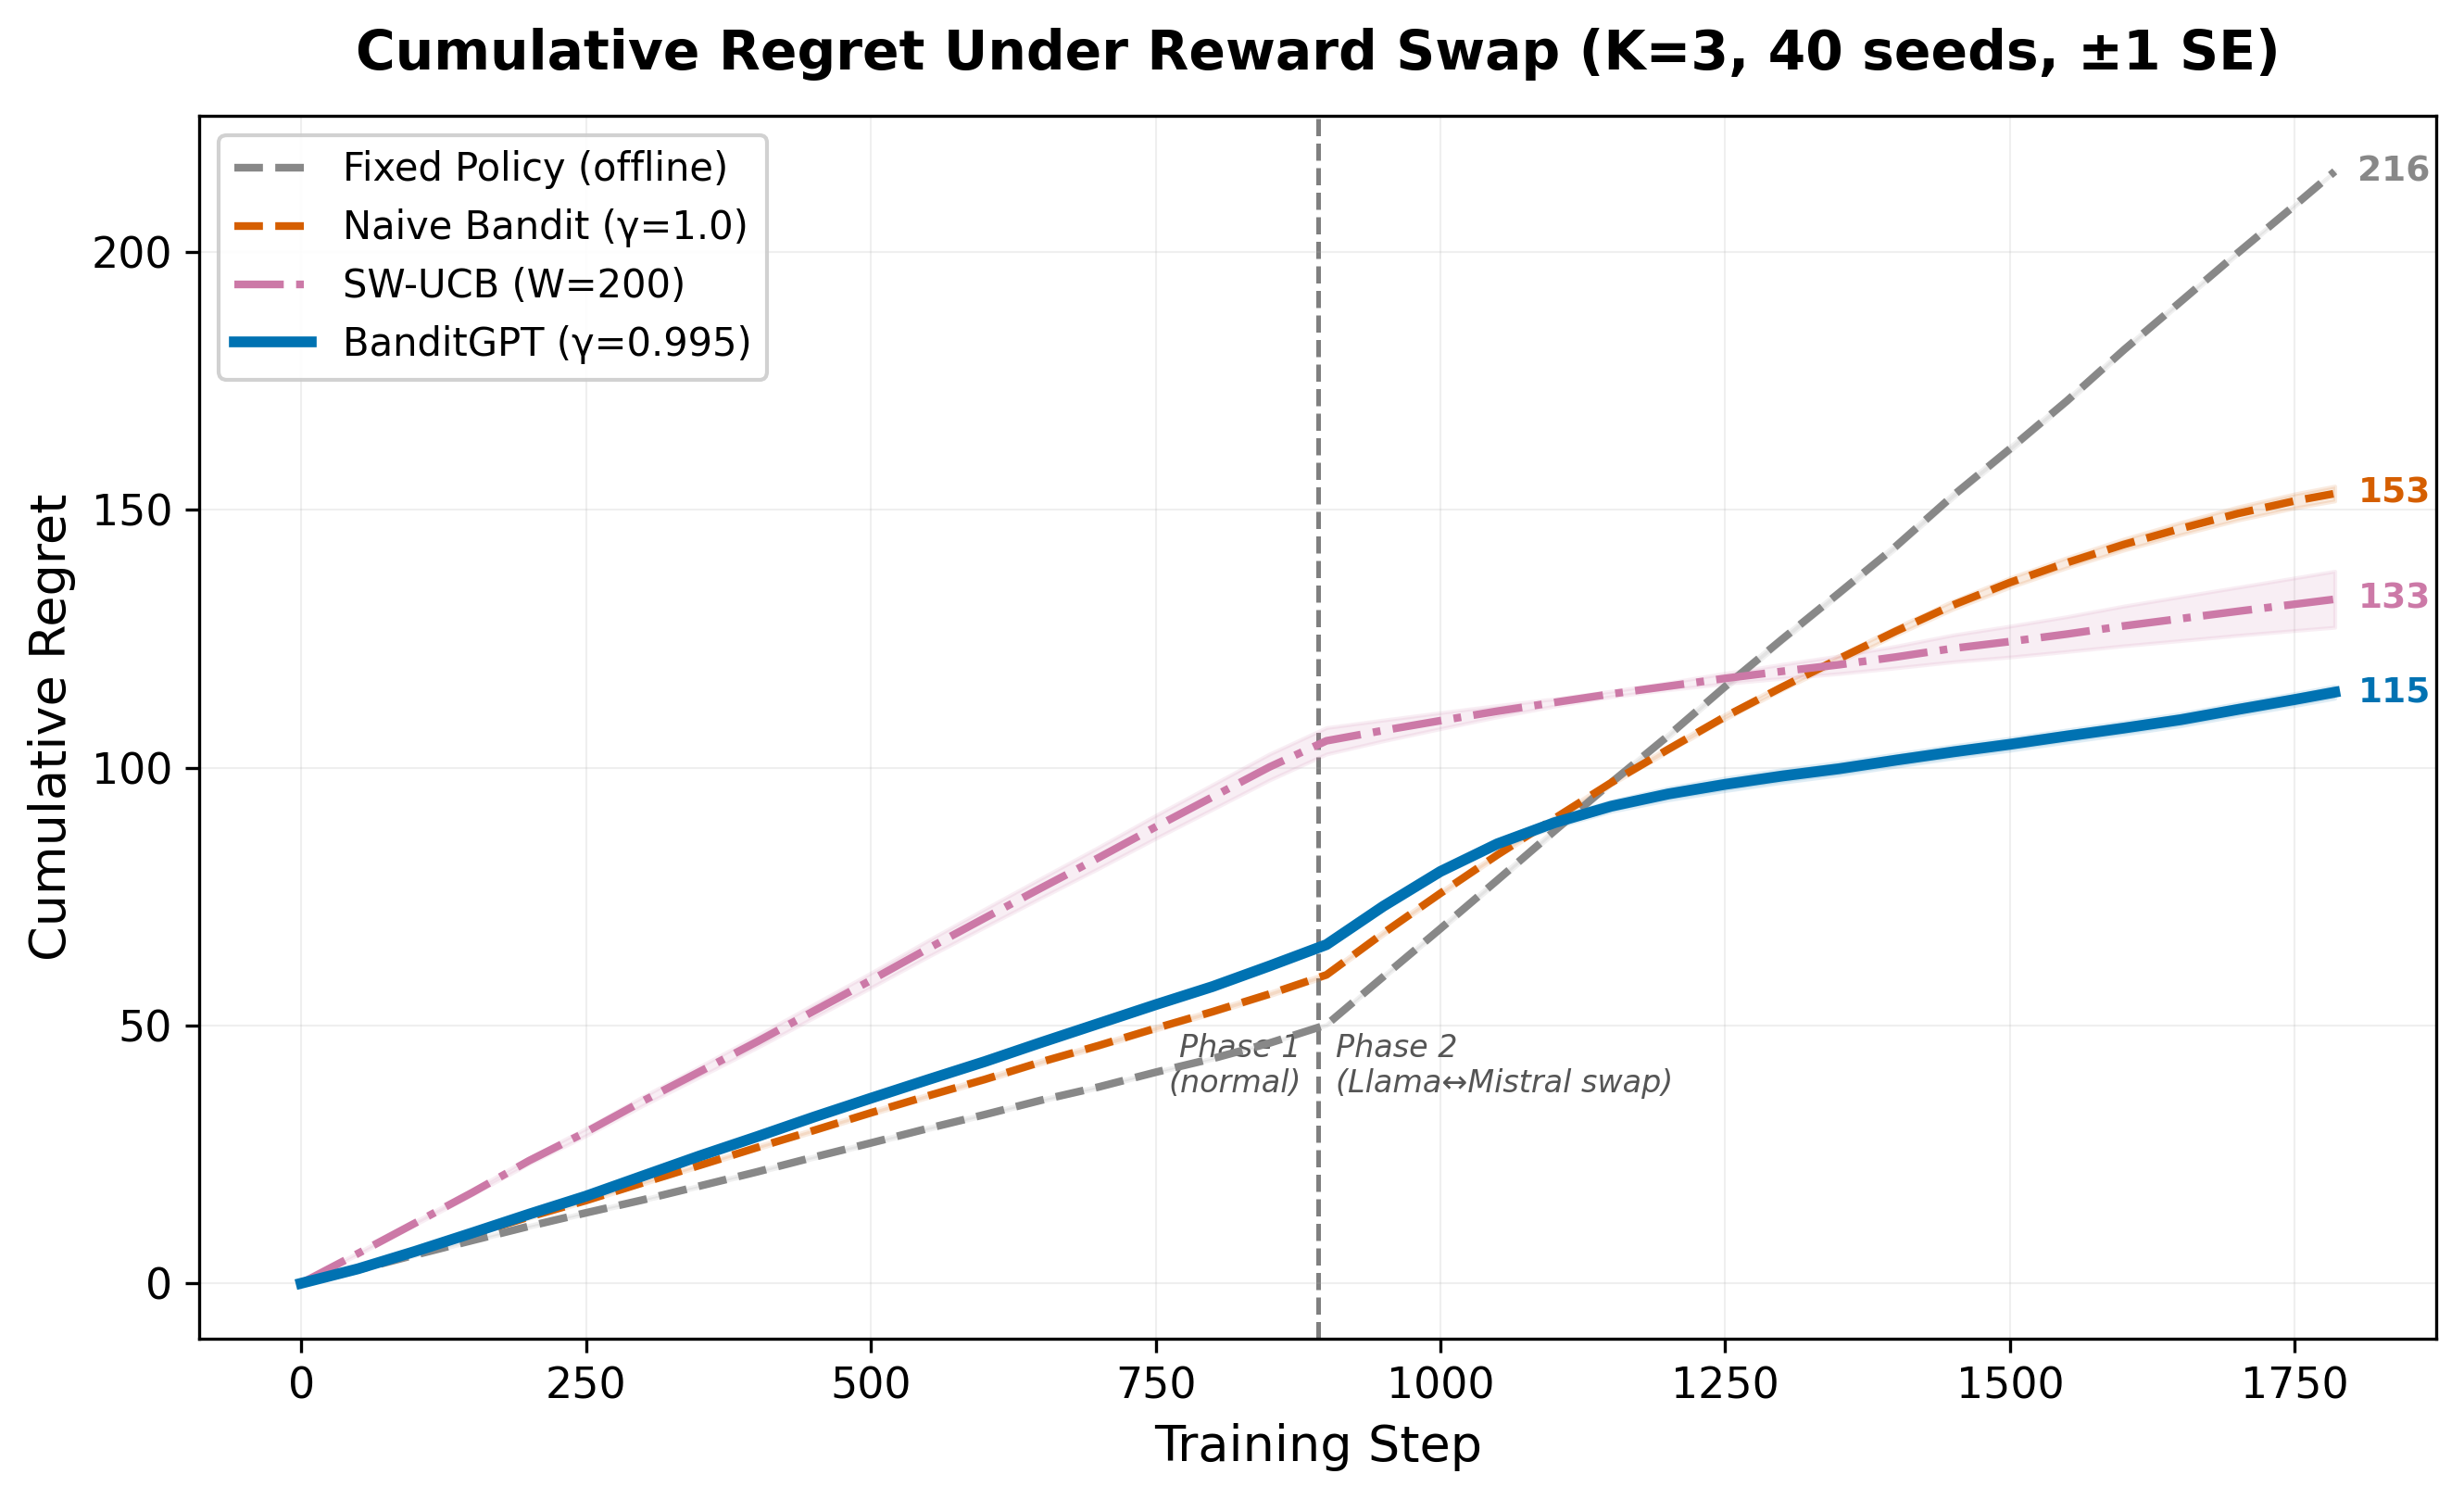
\includegraphics[width=\linewidth]{../experiments/02_nonstationary_k3_drift/results/cumulative_regret.pdf}
    \caption{Cumulative cost-adjusted regret under model quality shift
    ($K{=}3$; 40~seeds, $\pm$1\,SE shading).
    %
    Four conditions of increasing sophistication are compared:
    \textbf{Fixed Policy (offline)} deploys warmup priors without
    online learning.
    \textbf{Naive Bandit ($\gamma{=}1.0$)} adds online LinUCB
    with infinite memory.
    \textbf{SW-UCB ($W{=}200$)} uses sliding-window LinUCB without
    warmup priors.
    \textbf{BanditGPT ($\gamma{=}0.995$)} adds geometric
    forgetting with a tuned effective memory of ${\sim}200$ steps.
    %
    Total regret: Fixed~\rsFixedTotal{},
    Naive~\rsNaiveTotal{} ($-$\rsReductionFixedNaive\%),
    SW-UCB~\rsSWUCBTotal{},
    BanditGPT~\rsBanditGPTTotal{} ($-$\rsReductionNaiveBanditGPT\%
    vs.\ Naive).
    All pairwise comparisons are significant after
    Holm--Bonferroni correction (paired $t$-tests, 39~d.f.).
    }
    \label{fig:cumulative_regret}
\end{figure*}
